\documentclass[tikz]{standalone}
\usepackage{tikz}
\usetikzlibrary{mindmap,calc}
\usepackage{amsmath}
\usepackage{braket}

\begin{document}
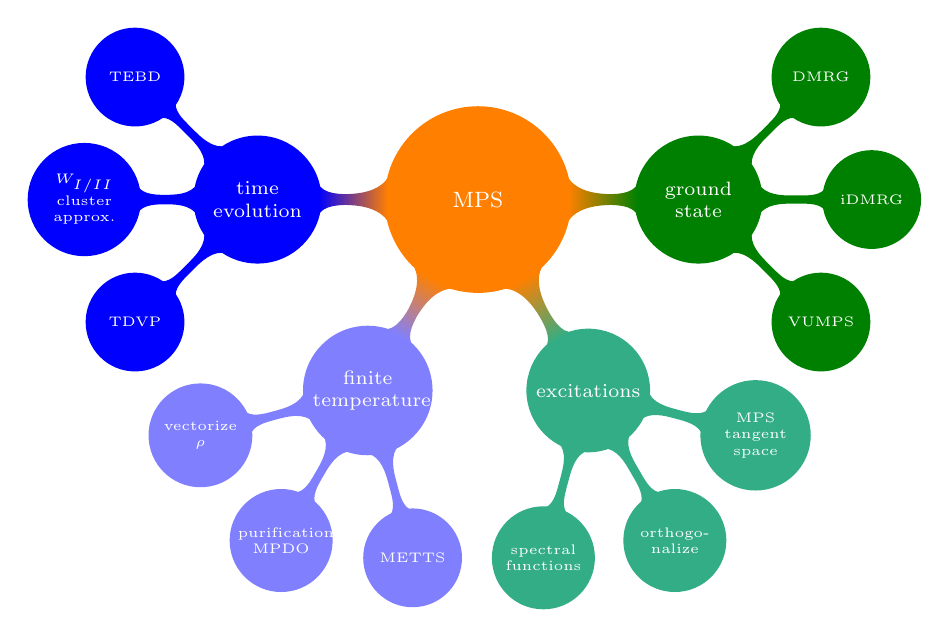
\begin{tikzpicture}
\begin{scope}[]
  \path[small mindmap,concept color=orange,text=white,
	  level 1 concept/.append style={sibling angle=60},
	  level 2 concept/.append style={sibling angle=45}]
    node[concept] {MPS}
	[clockwise from=0]
    % note that `sibling angle' can only be defined in
    % `level 1 concept/.append style={}'
    child[concept color=green!50!black] {
      node[concept] {ground state}
      [clockwise from=45]
      child { node[concept] {DMRG} }
      child { node[concept] {iDMRG} }
      child { node[concept] {VUMPS} }
    }
    child[concept color=green!60!blue!80] {
      node[concept] {excitations}
      [clockwise from=-15]
      child { node[concept] {MPS\\ tangent \\ space} }
      child { node[concept] {orthogo- \\nalize} }
      child { node[concept] {spectral\\ functions} }
    }
    child[concept color=blue!50] {
      node[concept] {finite \\temperature}
      [clockwise from=-75]
      child { node[concept] {METTS} }
      child { node[concept] {purification \\ MPDO} }
      child { node[concept] {vectorize \\$\rho$} }
    }
    child[concept color=blue] {
      node[concept] {time \\ evolution}
      [clockwise from=-135]
      child { node[concept] {TDVP} }
      child { node[concept] {$W_{I/II}$\\ cluster \\ approx.} }
      child { node[concept] {TEBD} }
    }
	;
\end{scope}
\end{tikzpicture}
\end{document}
